\chapterimage{chap39.jpg}
\chapter{Summary}


\section{双曲函数}

\begin{figure}[htbp]
	\centering
	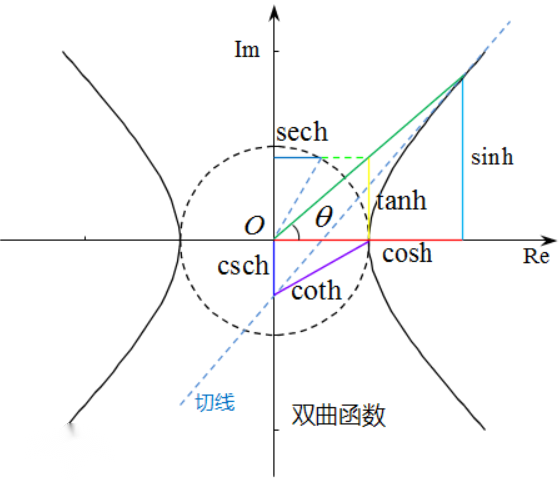
\includegraphics[width=9.5cm,height=8cm]{"figure/Summary/双曲函数.png"}
	\caption{双曲函数示意图}
	\label{Figure: 双曲函数示意图}
\end{figure} 
\begin{definition}\label{def: 双曲函数}
	双曲函数是一种类似于三角函数的一类函数,基本的函数有双曲正弦函数和双曲余弦函数,借由指数函数定义.
	
	1. 双曲正弦函数 
	$$\sinh x=\frac{e^{x}-e^{-x}}{2},x\in \mathbb{R}\quad \mathbb{R}\rightarrow \mathbb{R}$$
	
	2. 双曲余弦函数
	$$\cosh x=\frac{e^{x}+e^{-x}}{2},x\in \mathbb{R}\quad \mathbb{R}\rightarrow [1,+\infty]$$
	
	3. 双曲正切函数
	$$\tanh x=\frac{e^{x}-e^{-x}}{e^{x}+e^{-x}},x\in \mathbb{R}\quad \mathbb{R}\rightarrow (-1,1)$$
	
	恒等式:  
	$$\cosh^2 x-\sinh^2=1$$
	$$\sinh x=-i\sin ix,\quad \cosh x=\cos ix$$
	$$\sinh x=\sum\limits_{n=0}^{+\infty}\frac{x^{2n+1}}{(2n+1)!}=x+\frac{x^3}{3!}+\frac{x^5}{5!}+\dots$$
	$$\cosh x=\sum\limits_{n=0}^{+\infty}\frac{x^{2n}}{2n!}=1+\frac{x^2}{2!}+\frac{x^4}{4!}+\dots$$
\end{definition}
\begin{definition}
	反双曲函数:  
	
	1. 反双曲正弦函数
	$$\arsinh x=ln(x+\sqrt{x^2+1}),\quad (arsinh x)'=\frac{1}{\sqrt{x^2+1}}$$
	
	2. 反双曲余弦函数
	$$\arcosh x=ln(x+\sqrt{x^2-1}),\quad (arcosh x)'=\frac{1}{\sqrt{x^2-1}}$$
	
	3. 反双曲正切函数
	$$\artanh x=\frac{1}{2}ln(\frac{1+x}{1-x}),\quad (artanh x)'=\frac{1}{1-x^2}$$
\end{definition}


\section{特殊曲线}

\begin{definition}\label{def: 常用曲线}
	几类特殊曲线的面积、弧长、旋转体体积
	
	1.心形线 \quad $r=a(1+\cos \theta)$
	$$L=\int_{0}^{2\pi}\sqrt{a^2(1+\cos \theta)^2+a^2\sin^2\theta}d\theta=8a$$
	$$S=2\int_{0}^{\pi}a^2(1+\cos \theta)^2d\theta=\frac{3}{2}a^2\pi$$
	
	2.摆线\quad 
	$\left\lbrace
	\begin{array}{l}
		x=a(\theta-\sin \theta)\\
		y=a(1-\cos \theta)
	\end{array}
	 \right. $
	 $$L=\int_{0}^{2\pi}\sqrt{a^2(1-\cos \theta)^2+a^2\sin^2\theta}d\theta=8a$$
	 $$S=\int_{0}^{x_{0}}f(x)dx=\int_{0}^{2\pi}a^2(1-\cos \theta)^2d\theta=3a^2\pi$$
	
	3.星形线\quad $x^{\frac{2}{3}}+y^{\frac{2}{3}}=a^{\frac{2}{3}}\Leftrightarrow$
	$\left\lbrace
	\begin{array}{l}
		x=a\cos^3\theta\\
		y=a\sin^3\theta
	\end{array}
	 \right. $
	$$L=4\int_{0}^{\frac{\pi}{2}}3a\sin\theta\cos\theta d\theta=6a$$
	$$S=4\int_{0}^{\frac{\pi}{2}}3a\sin^4\theta\cos^2\theta=\frac{3\pi}{8}a^2$$
	
	4.三叶玫瑰线 \quad $\rho=a\cos 3\theta$\quad $\rho=a\sin 3\theta$
	$$L=3\int_{\frac{\pi}{6}}^{\frac{\pi}{2}}\sqrt{a^2\cos^2 3\theta+9a^2\sin^2 3\theta}d\theta=2a\int_{0}^{\frac{\pi}{2}}\sqrt{1+8\sin^2 t}dt$$
	$$S=\frac{3}{2}\int_{\frac{\pi}{6}}^{\frac{\pi}{2}}a^2\cos^2 3\theta d\theta=\frac{\pi a^2}{4}$$
	
	5.伯努利双扭线\quad $\rho^2=a^2\cos 2\theta$
	$$L=4\int_{0}^{\frac{\pi}{4}}a\sqrt{\frac{\sin^2 2\theta}{\cos 2\theta}+\cos^2 2\theta}=2a\int_{0}^{\frac{\pi}{2}}\cos^{-\frac{1}{2}}\theta d\theta$$
	$$S=2\int_{0}^{\frac{\pi}{4}}a^2\cos 2\theta d\theta=a^2$$
\end{definition}
\begin{figure}[H]
	\centering  %图片全局居中
	\subfigure[心形线]{
	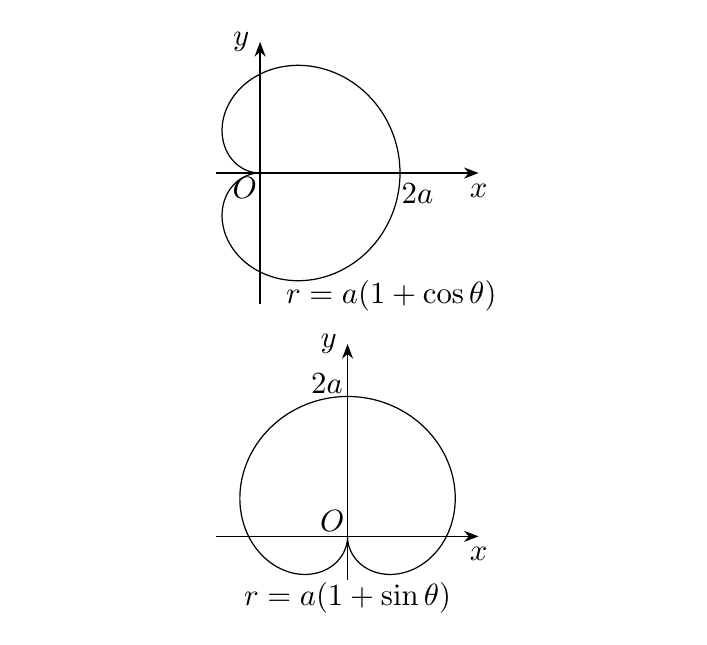
\includegraphics[width=0.45\textwidth]{"figure/Summary/心形线.png"}}
	\subfigure[摆线]{
	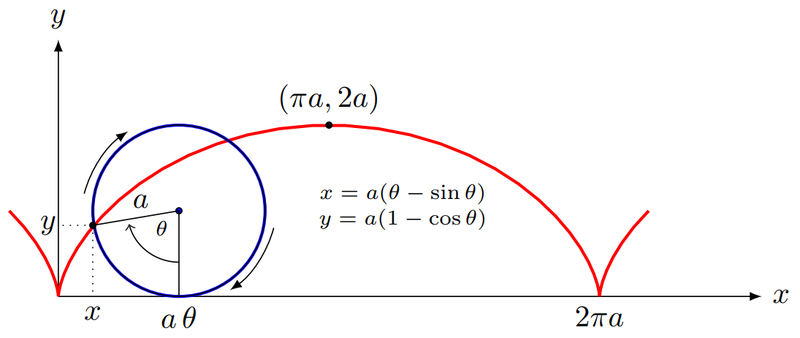
\includegraphics[width=0.45\textwidth]{"figure/Summary/摆线.png"}}
	\subfigure[星形线]{
	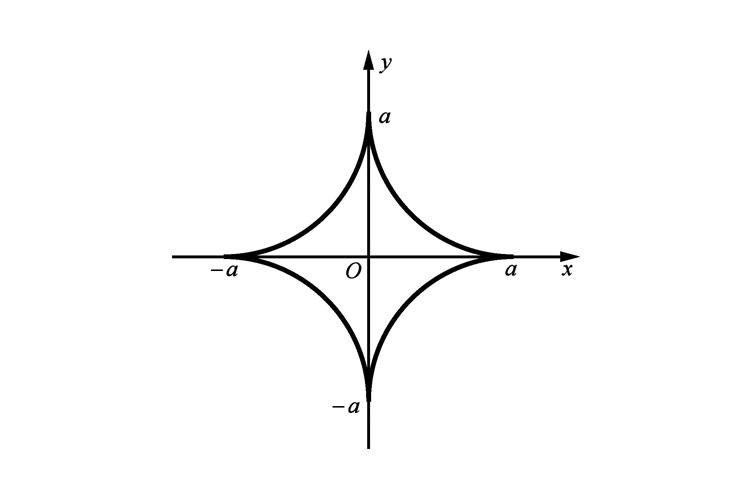
\includegraphics[width=0.45\textwidth]{"figure/Summary/星形线.jpg"}}
	\subfigure[三叶玫瑰线$\rho=a\cos 3\theta$]{
	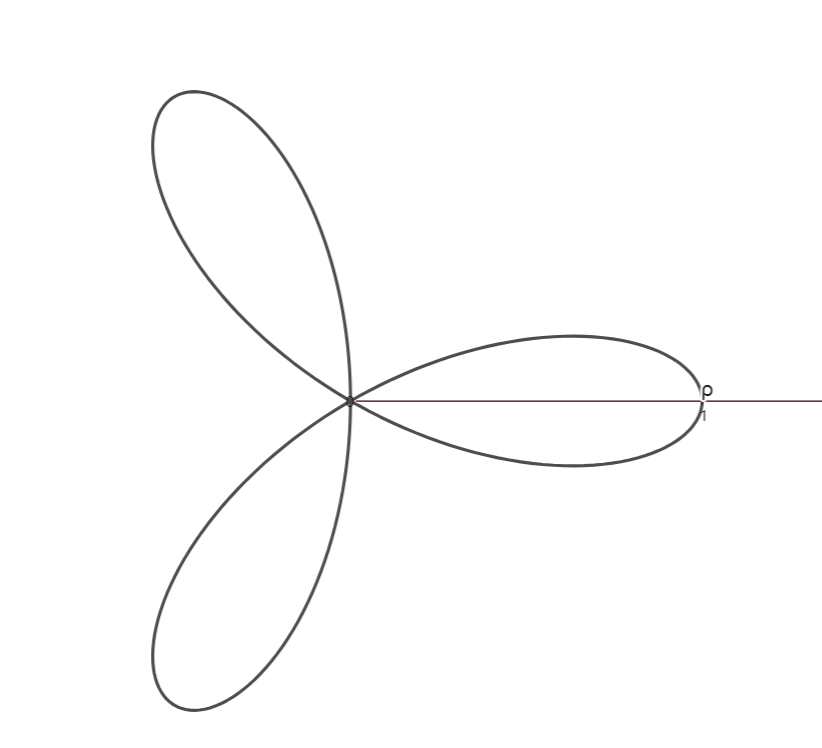
\includegraphics[width=0.45\textwidth]{"figure/Summary/三叶玫瑰线1.png"}}
	\subfigure[三叶玫瑰线$\rho=a\sin 3\theta$]{
	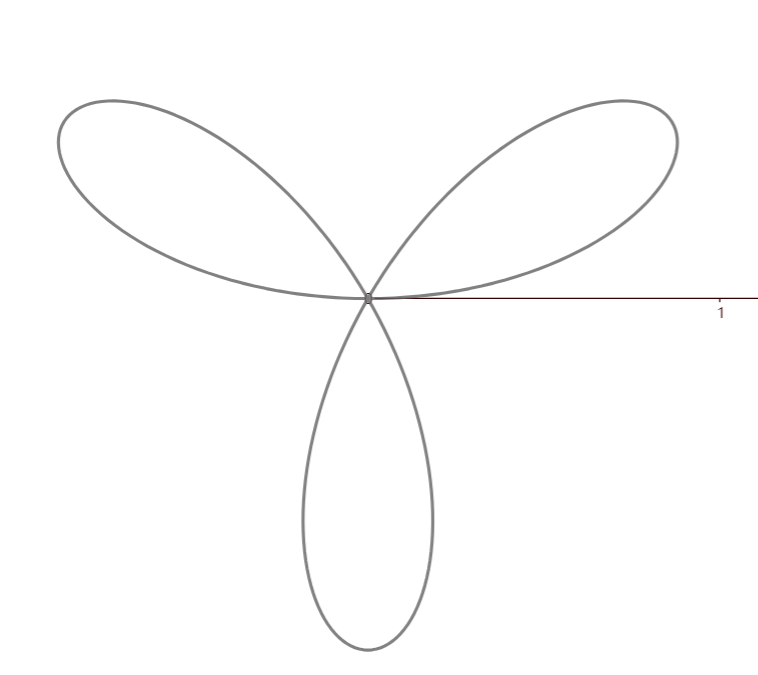
\includegraphics[width=0.45\textwidth]{"figure/Summary/三叶玫瑰线2.png"}}
	\subfigure[伯努利双扭线$\rho^2=a^2\cos 2\theta$]{
	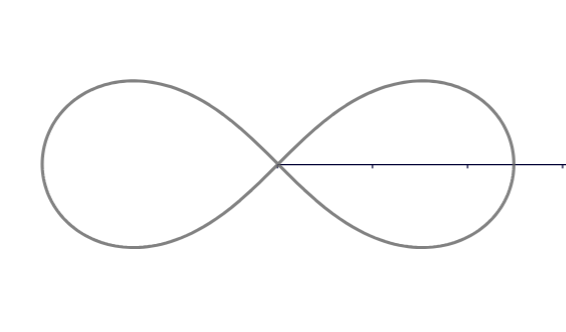
\includegraphics[width=0.45\textwidth]{"figure/Summary/伯努利双扭线.png"}}
	\caption{曲线图形}
\end{figure}

\section{两类欧拉积分}

\begin{definition}[$Gamma$ 函数和 $Beta$函数]	
	1. $Gamma$ 函数(欧拉第一类积分)
	$$B(p,q)=\int_{0}^{1}x^{p-1}(1-x)^{q-1}dx=B(q,p)$$
	
	我们有:  $$B(a,b)=(\frac{x^a(1-x)^b}{a})|_{0}^{1}+\frac{b-1}{a}\int_{0}^{1}x^{a}(1-x)^{b-2}dx$$
	$$B(a,b)=\frac{b-1}{a}\int_{0}^{1}(x-1+1)x^{a-1}(1-x)^{b-2}$$
	$$\mathcolorbox{yellow}{B(a,b)=\frac{b-1}{a}[B(a,b-1)-B(a,b)]}$$ $$\mathcolorbox{yellow}{B(a,b)=\frac{b-1}{a+b-1}B(a,b-1)}$$
	
	特别的,我们有:  $$\mathcolorbox{yellow}{B(m,n)=\frac{(n-1)!(m-1)!}{(m+n-1)!}}$$
	
	2.$Beta$函数(第二类欧拉积分)
	$$\Gamma(\alpha)=\int_{0}^{+\infty}x^{\alpha-1}e^{-x}dx$$
	
	我们有:  $$\Gamma(\alpha)=(-x^{\alpha-1}e^{-x})|_{0}^{+\infty}+(\alpha-1)\int_{0}^{+\infty}x^{\alpha-2}e^{-x}dx$$
	$$\mathcolorbox{red}{\Gamma(\alpha)=(\alpha-1)\Gamma(\alpha-1)},\alpha>1$$
	
	特别的,我们有:  $$\mathcolorbox{red}{\Gamma(n+1)=n!}$$
	
	3. 两类积分之间的关系
	
	转换公式:  
	$$B(a,b)=\frac{\Gamma(a)\Gamma(b)}{\Gamma(a+b)}$$
	
\end{definition}


\section{谱分解定理}

\begin{definition}[代数重复度]
	设$\lambda_{1},\lambda_{2},\cdots,\lambda_{k}$是矩阵$A\in \mathbb{C}^{n\times n}$的相异特征值,其重数分别为$r_{1},r_{2},\cdots,r_{k}$,称$r_{i}$为矩阵$A$的特征值$\lambda_{i}$的代数重复度.
\end{definition}
\begin{definition}[几何重复度]
	齐次方程组$Ax=\lambda_{i}x\ (i=1,2,\cdots,k)$的解空间$V_{\lambda_{i}}$称为$A$的对应于特征值$\lambda_{i}$的特征空间,则$V_{\lambda_{i}}$的维数称为$A$的特征值$\lambda_{i}$的几何重复度.
\end{definition}
\begin{definition}[单纯矩阵]
	若矩阵$A$的每一个特征值的代数重复度与几何重复度相等,则称矩阵$A$为单纯矩阵.
\end{definition}
\begin{definition}[幂等矩阵]
	若$A$为方阵,且$A^2=A$,则称$A$为幂等矩阵.
\end{definition}
\begin{property}[幂等矩阵$A$性质]
	\begin{itemize}
		\item (1). $A$是单纯矩阵,且其$Jordan$标准型为$\left(\begin{matrix}
			I_{r}&0\\0&0
		\end{matrix} \right) $
		\item (2). $A$的特征值只能为$0$或者$1$
		\item (3). $rank(A)=tr(A)$
		\item (4). $Ax=x\Leftrightarrow x\in\mathbb{R}(A)$
		\item (5). $A$一定可以相似对角化
	\end{itemize}
\end{property}
\begin{theorem}[谱分解定理]\label{the: 谱分解定理}
	设$A\in\mathbb{C}^{n\times n}$是单纯矩阵,矩阵$A$有$k$个相异特征值$\lambda_{i}\ (i=1,2,\cdots,k)$,$\exists A_{i}\in \mathbb{C}^{n\times n}\ (i=1,2,\cdots,k)$,使得
	$$A=\sum\limits_{i=1}^{k}\lambda_{i}G_{i}$$
	
	此式称为矩阵$A$的谱分解,$G_{1},G_{2},\cdots,G_{k}$称为$A$的族谱,且满足一下性质:  
	\begin{property}[谱分解谱族$G_{i}$性质]
		\begin{itemize}
			\item (1). 幂等性:  $G_{i}^2=G_{i}$
			\item (2). 分离性:  $G_{i}G_{j}=0\ (i\neq j)$
			\item (3). 可加性:  $\sum\limits_{i=1}^{k}G_{i}=E_{n}$
		\end{itemize}
	\end{property}
	\begin{corollary}[谱族$G_{i}$推论]
		\begin{itemize}
			\item $AG_{i}=G_{i}A=\lambda_{i}G_{i}$
			\item $rank(G_{i})=m_{i}$
			\item $G_{i}$是唯一的,$G$的族谱是唯一的.
		\end{itemize}
	\end{corollary}
	\begin{proposition}
		矩阵$A$是单纯矩阵等价为存在$k$个矩阵$G_{i},\ (i=1,2,\cdots,k)$满足:  
		\begin{itemize}
			\item (1). $G_{i}G_{j}=\left\lbrace
			\begin{array}{l}
				G_{i},\ i=j\\0,\ i\neq j
			\end{array}
			\right. $
			\item (2). $\sum\limits_{i=1}^{k}G_{i}=E_{n}$
			\item (3). $A=\sum\limits_{i=1}^{k}\lambda_{i}G_{i}$
			\item (4). $f(A)$为任意多项式,则$$f(A)=\sum\limits_{i=1}^{k}f(\lambda_{i})G_{i}$$
			\item (5). $A^m=\sum\limits_{i=1}^{k}\lambda_{i}^mG_{i}$
		\end{itemize}
	\end{proposition}
\end{theorem}
\begin{anymark}[证明]
	1. 必要性
	 
	(1). 当$k=n$时:  
	
	我们由$A$是单纯矩阵可以得到矩阵$A$可以相似对角化
	$$A=P\Lambda P^{-1},\text{其中}\Lambda=diag\{\lambda_{1},\lambda_{2},\cdots,\lambda_{n}\}$$
	
	我们不妨设$P=(v_{1},v_{2},\cdots,v_{n})$,$P^{-1}=\left( \begin{matrix}
		\omega_{1}^{T}\\\omega_{2}^{T}\\ \vdots\\\omega_{n}^{T}
	\end{matrix}\right) $,我们可以得到:  
	$$A=(v_{1},v_{2},\cdots,v_{n})\left[\begin{matrix}
		\lambda_{1}&0&\cdots&0\\
		0&\lambda_{2}&\cdots&0\\
		\cdots&\cdots&\cdots&\cdots\\
		0&0&\cdots&\lambda_{n}
	\end{matrix} \right] \left( \begin{matrix}
		\omega_{1}^{T}\\\omega_{2}^{T}\\ \vdots\\\omega_{n}^{T}
	\end{matrix}\right) \Rightarrow A=\sum\limits_{i=1}^{n}\lambda_{i}v_{i}\omega_{i}^{T}=\sum\limits_{i=1}^{n}\lambda_{i}G_{i},\ \text{其中}G_{i}=v_{i}\omega_{i}^{T}$$
	
	我们由$\left\lbrace
	\begin{array}{l}
		P^{-1}P=E_{n}\\
		PP^{-1}=E_{n}
	\end{array}
	\right.\Rightarrow\left\lbrace
	\begin{array}{l}
		\omega_{i}^{T}v_{j}=\left\lbrace
		\begin{array}{l}
			1,\ i=j\\
			0,\ i\neq j
		\end{array}
		\right. \\
		\sum\limits_{i=1}^{n}v_{i}\omega_{i}^{T}=\sum\limits_{i=1}^{n}G_{i}=E_{n}
	\end{array}
	\right.$
	
	对于任意$i,j\in(1,n),G_{i}G_{j}=v_{i}(\omega_{i}^{T}v_{j})\omega_{j}^{T}$,我们可以得到:  
	$$G_{i}G_{j}=\left\lbrace
	\begin{array}{l}
		v_{i}\omega_{i}^{T}=G_{i},\ i=j\\
		0,\ i\neq j
	\end{array}
	\right. \Rightarrow A_{i}\text{是幂等矩阵}$$
	
	(2). 当$k<n$时:  
	
	我们由矩阵$A$是单纯矩阵,可以得到:  $A=P\Lambda P^{-1}$
	$$\left\lbrace
	\begin{array}{l}
		P=(v_{11},v_{12},\cdots,v_{1r_{1}},v_{21},v_{22},\cdots,v_{2r_{2}},\cdots,v_{k1},v_{k2},\cdots,v_{kr_{k}})\\
		P^{-1}=(\omega_{11}^{T},\omega_{12}^{T},\cdots,\omega_{1r_{1}}^{T},\omega_{21}^{T},\omega_{22}^{T},\cdots,\omega_{2r_{2}}^{T},\cdots,\omega_{k1}^{T},\omega_{k2}^{T},\cdots,\omega_{kr_{k}}^{T})^{T}
	\end{array}
	\right. $$
	$$A=\sum\limits_{i=1}^{k}\lambda_{i}\sum\limits_{j=1}^{r_{i}}B_{ij}\stackrel{G_{i}=\sum\limits_{j=1}^{r_{i}}B_{ij}}{\longrightarrow}A=\sum\limits_{i=1}^{k}\lambda_{i}G_{i}$$
	$$P^{-1}P=E_{n}\Rightarrow \omega_{ij}^{T}v_{lk}=\left\lbrace
	\begin{array}{l}
		1,\ i=l,j=k\\
		0,\ i\neq l\text{或}j\neq k
	\end{array}
	\right. $$
	$$B_{ij}B_{lk}=v_{ij}(\omega_{ij}^{T}v_{lk})\omega_{lk}^{T}=\left\lbrace
	\begin{array}{l}
		B_{ij},\ i=l,j=k\\
		0,\ i\neq l\text{或}j\neq k
	\end{array}
	\right. \Rightarrow G_{i}G_{j}=\sum\limits_{p=1}^{r_{i}}B_{ip}\sum\limits_{q=1}^{r_{j}}B_{jq}=\left\lbrace
	\begin{array}{l}
		G_{i},\ i=j\\0,\ i\neq j
	\end{array}
	\right. $$
	$$\sum\limits_{i=1}^{k}G_{i}=\sum\limits_{i=1}^{n}B_{i}=E_{n}$$
	(2). 充分性
	
	我们首先可以得到矩阵$G_{i}$均为幂等矩阵,我们不妨设$dim\mathbb{R}(G_{i})=n_{i}$,我们可以得到:  
	$$n_{i}=tr(G_{i})\Rightarrow \sum\limits_{i=1}^{k}n_{i}=\sum\limits_{i=1}^{k}tr(G_{i})=tr(\sum\limits_{i=1}^{k}G_{i})=tr(E_{n})=n$$
	
	我们取$X_{i}$为$\mathbb{R}(G_{i})$的基列构成的阵,则$X=(X_{1},X_{2},\cdots,X_{k})$是$n\times n$矩阵,且$G_{i}$的列向量都可以由$X_{i}$线性表出,我们可以得到:  
	$$G_{i}=(X_{i}\beta_{1},X_{i}\beta_{2},\cdots,X_{i}\beta_{n})=X_{i}Y_{i}$$
	$$XY=(X_{1},X_{2},\cdots,X_{n})\left( \begin{matrix}
		Y_{1}\\Y_{2}\\\vdots\\Y_{n}
	\end{matrix}\right)=\sum\limits_{i=1}^{n}X_{i}Y_{i}=E_{n}\Rightarrow \text{矩阵}X\text{可逆}$$

	$$YX=\left( \begin{matrix}
		Y_{1}\\Y_{2}\\\vdots\\Y_{n}
	\end{matrix}\right)(X_{1},X_{2},\cdots,X_{k})=\left[ \begin{matrix}
	Y_{1}\\Y_{2}\\\cdots\\Y_{k}
\end{matrix}\right] =\left[\begin{matrix}
Y_{1}X_{1}&Y_{1}X_{2}&\cdots&Y_{1}X_{k}\\
Y_{2}X_{1}&Y_{2}X_{2}&\cdots&Y_{2}X_{k}\\
\cdots&\cdots&\cdots&\cdots\\
Y_{k}X_{1}&Y_{k}X_{2}&\cdots&Y_{k}X_{k}\\
\end{matrix} \right] =E_{n}=\left[\begin{matrix}
E_{r_{1}}&0&\cdots&0\\
0&E_{r_{2}}&\cdots&0\\
\cdots&\cdots&\cdots&\cdots\\
0&0&\cdots&E_{r_{k}}\\
\end{matrix} \right]$$

我们可以得到:  
$$Y_{i}X_{j}=\left\lbrace
\begin{array}{l}
	E_{r_{i}},\ i=j\\
	0,\ i\neq j
\end{array}
\right. \Rightarrow G_{i}X_{j}=x_{i}Y_{i}X_{j}=\left\lbrace
\begin{array}{l}
	X_{i},\ i=j\\
	0,\ i\neq j
\end{array}
\right. $$

	我们利用幂等矩阵的性质
	\begin{eqnarray*}
		AX&=&(\sum\limits_{i=1}^{k}\lambda_{i}G_{i})(X_{1},X_{2},\cdots,X_{k})\\
		&=&((\sum\limits_{i=1}^{k}\lambda_{i}G_{i})X_{1},(\sum\limits_{i=1}^{k}\lambda_{i}G_{i})X_{2},\cdots,(\sum\limits_{i=1}^{k}\lambda_{i}G_{i})X_{k})\\
		&=&(\lambda_{1}X_{1},\lambda_{2}X_{2},\cdots,\lambda_{k}X_{k})\\
		&=&(X_{1},X_{2},\cdots,X_{k})\left[\begin{matrix}
			E_{r_{1}}&0&\cdots&0\\
			0&E_{r_{2}}&\cdots&0\\
			\cdots&\cdots&\cdots&\cdots\\
			0&0&\cdots&E_{r_{k}}\\
		\end{matrix} \right]\\
	&=&X\Lambda\Rightarrow A=X\Lambda X^{-1} 
	\end{eqnarray*}
	
	(3). 谱分解唯一性
	
	我们不妨假设$F_{1},F_{2},\cdots,F_{k}$满足:  
	$$\left\lbrace
	\begin{array}{l}
		F_{i}F_{j}=0,\ i\neq j\\
		F_{i}^2=F_{i}\\
		A=\sum\limits_{i=1}^{k}\lambda_{i}F_{i}\\
		\sum\limits_{i=1}^{k}F_{i}=E_{n}
	\end{array}
	\right. $$
	
	我们由族谱$G_{i}$性质推论可以得到:  
	$$\left\lbrace
	\begin{array}{l}
		AG_{i}=G_{i}A=\lambda_{i}G_{i}\\
		AF_{i}=F_{i}A=\lambda_{i}F_{i}
	\end{array}
	\right. \Rightarrow \left\lbrace
	\begin{array}{l}
		AG_{i}F_{j}=\lambda_{i}G_{i}F_{j}\\
		\lambda_{i}G_{i}F_{j}=G_{i}AF_{j}\\
		G_{i}AF_{j}=\lambda_{j}G_{i}F_{j}
	\end{array}
	\right. \Rightarrow G_{i}F_{j}=0,\ i\neq j$$
	
	我们得到:  $$G_{i}=G_{i}E_{n}=G_{i}(\sum\limits_{j=1}^{k}F_{j})=G_{i}F_{i}=(\sum\limits_{j=1}^{k}G_{j})F_{i}=F_{i}$$
	
	综上所述,矩阵$A$的谱分解是唯一的.
\end{anymark}
\myspace{1}


\section{多项式函数极值点和拐点}


\begin{theorem}[代数基本定理]\label{the: 代数基本定理}
	任何一个一元 $n$ 次复系数多项式, 都恰好有 $n$ 个复根, 且可以表示为 $n$ 个一次因式的乘积.
\end{theorem}

\begin{corollary}[曲线的极值点和拐点]
	曲线上的可导点不可能同时是极值点和拐点, 不可导点可能同时是极值点和拐点.
\end{corollary}

\begin{proposition}[多项式函数极值点和拐点个数:命题一]\label{pro: 命题一}
	多项式函数 $f(x) = (x-a)^{n},(n>1)$, 当 $n$ 为奇数时, $(a,0)$ 是 $f(x)$ 的拐点, 当 $n$ 为偶数时, $x=a$ 是 $f(x)$ 的极值点.
\end{proposition}
\begin{anymark}[证明]

	$$f'(x) = n(x-a)^{n-1},\quad f''(x) = n(n-1)(x-a)^{n-2}$$
	当 $n$ 为偶数时, 我们有: $f'(a) = 0$ 且 
	$$\exists x\in \mathring{U}(a,\delta), f(x) = (x-a)^{n} > 0 = f(a)$$

	或者 
	$$\exists \delta > 0, x\in (a-\delta,a),f'(x)<0; x\in (a,a+\delta),f'(x)>0$$
	
	我们有: 当 $n$ 为偶数时, $x=a$ 是 $f(x)$ 的极值点.
	
	当 $n$ 为奇数时, 我们有: $f''(a) = 0$ 且
	
	$$\exists \delta > 0, x\in (a-\delta,a),f''(x)<0; x\in (a,a+\delta),f''(x)>0$$

	我们有: 当 $n$ 为奇数时, $(a,0)$ 是 $f(x)$ 的拐点.
	

\end{anymark}


\begin{proposition}[多项式函数极值点和拐点个数:命题二]\label{pro: 命题二}
	多项式函数 $f(x) = (x-a)^{n}g(x), (n>1), g(a)\neq 0$, 当 $n$ 为奇数时, $(a,0)$ 是 $f(x)$ 的拐点, 当 $n$ 为偶数时, $x=a$ 是 $f(x)$ 的极值点.
\end{proposition}
\begin{anymark}[证明]

	$$\begin{cases}
		f'(x) = ng(x)(x-a)^{n-1} + g'(x)(x-a)^{n} = (x-a)^{n-1}[ng(x)+(x-a)g'(x)]\\
		f''(x) = (x-a)^{n-2}[n(n-1)g(x) +2n(x-a)g'(x)+(x-a)^{2}g''(x)]
	\end{cases}$$

	当 $n$ 为偶数时, 我们不妨假设 $g(a) > 0$, 根据极限的保号性,我们有:
	$$\exists \delta_{1} > 0, s.t.\ x\in U(a,\delta_{1}), g(a) > 0$$
	
	当 $x\in U(a,\delta_{1}), f(x) = (x-a)^{n}g(x) \geq f(a) =0$, $x=a$ 是 $f(x)$ 的一个极值点. 


	当 $n$ 为奇数时, $x\to a,(x-a),(x-a)^{2}$都是无穷小量, $g'(a),g''(a)$ 都是定值, 因此
	$$\exists \delta_{2} > 0, s.t.\ x\in U(a,\delta_{2}), 2n(x-a)g'(x)+(x-a)^{2}g''(x)\leq |n(n-1)g(x)| $$

	我们有: $x\in U(a,\delta_{2}), [n(n-1)g(x) +2n(x-a)g'(x)+(x-a)^{2}g''(x)] > 0$, 即: $f''(x)$ 与 $(x-a)^{n-2}$ 符号相同

	当 $x\in (a-\delta_{2},a), f''(x) < 0; x\in (a,a+\delta_{2}), f''(x) > 0$, $(a,0)$ 是 $f(x)$ 的一个拐点.
\end{anymark}

\begin{proposition}[多项式函数极值点和拐点个数:命题三]\label{pro: 命题三}
	讨论多项式函数: $P_{n}(x) = \prod\limits_{i=1}^{k}(x-a_{i})^{p_{i}}$ 极值点和拐点个数,其中满足:
	$$a_{i}\in\mathbb{R}, a_{1}<a_{2}<\cdots<a_{k}, p_{i}\in \mathbb{Z}^{+}$$
\end{proposition}

\begin{anymark}[证明]
	我们首先有: $P_{n}(x)$ 是多项式函数, 在 $\mathbb{R}$ 上 $n$ 阶可导, $P_{n}(x)$ 的极值点一定满足: $P_{n}'(x) = 0$, 拐点满足: $P_{n}''(x) = 0$
	\myspace{1}

	$P(x)$ 有 $k$ 个实数根, 这 $k$ 个实数根的重数分别为: $p_{1},p_{2},\cdots,p_{k}$, 且 $\sum\limits_{i=1}^{k}p_{i}= n$

	我们利用多个函数连乘的求导公式:
	$$P_{n}'(x) =  \prod\limits_{i=1}^{k}(x-a_{i})^{p_{i}-1}\left[\sum\limits_{i=1}^{k}p_{i}\left(\prod\limits_{j=1\\j\neq i}^{k}(x-a_{j})\right)\right]$$

	当 $p_{i} \geq 2 (i = 1,2,\cdots,k)$ 时, $x=a_{i}(i=1,2,\cdots,k)$ 是 $P_{n}'(x)$ 的一个零点,此类的驻点一共有 $k$ 个, $P_{n}'(x)$ 有 $p_{i}-1 (i=1,2,\cdots,k)$ 重根 $a_{i}(i=1,2,\cdots,k)$
	\myspace{1}
	$P_{n}'(x)$ 此类的零点个数为: $n_{1} = \sum\limits_{i=1}^{k}(p_{i}-1) = n-k$
	\myspace{1}
	在 $(a_{i},a_{i+1}),(i=1,2,\cdots,k-1)$ 中, 我们由罗尔定理得到: $\exists \xi_{i}\in(a_{i},a_{i+1}),(i=1,2,\cdots,k-1), s.t.\ P'(\xi_{i}) = 0$, 此类零点的个数为 $k-1$ 个
	\myspace{1}
	$P'_{n}(x)$ 是 $n-1$ 次多项式函数, 至多有 $n-1$ 个复根, 我们得到 $P'_{n}(x)$ 有 $n-k+k-1 = n-1$ 个实数根, 其中前面 $n-k$ 个根中存在重根情况.
	\begin{corollary}[多项式函数零点]
		$P_{n}(x)$ 有 $n$ 个实数根(含重根), 那么 $P_{n}'(x),P_{n}''(x),\cdots,P_{n}^{(n-1)}(x)$ 的根全部是实数.
	\end{corollary}

	我们继续看 $P_{n}'(x)$ 的两类零点, 其中一类是 $x=a_{i}(i=1,2,\cdots,k),(p_{i}>1)$, 另一类是 $x=\xi_{i}(i=1,2,\cdots,k-1)$
	\myspace{1}
	第一类零点:我们由 $\mathbf{pro: }$ \ref{pro: 命题二}得到: 当 $p_{i}$ 为偶数的时候, $a_{i}$ 是 $P_{n}(x)$ 的极值点, 当 $p_{i}$ 为奇数的时候, $a_{i}$ 是 $P_{n}(x)$ 的拐点
	\myspace{1}
	第二类零点: $P_{n}'(x) = \sum\limits_{i=1}^{n-1}(x-\eta_{i}),\eta_{i}\in\mathbb{R}$, 当 $x\in U(\xi_{i},\delta)$ 时, 只有 $(x-\xi_{i})$ 这一项符号改变, 因此 $x=\xi_{i}$ 是 $P_{n}(x)$ 极值点
	\myspace{1}
	我们不妨假设 $p_{i} > 1\ \&\ p_{i}\text{为奇数}$ 的个数为 $k_{1}$, $p_{i} > 1\ \&\ p_{i}\text{为偶数}$ 的个数为 $k_{2}$
	\myspace{1}
	$P_{n}(x)$ 的极值点个数为 $k-1+k_{2}$

	\myspace{2}
	关于拐点的个数,我们可以类比极值点个数的方法, 将 $P_{n}'(x)$ 当做原函数,求 $P_{n}'(x)$ 的极值点个数, 我们将 $P_{n}'(x)$改写为:
	
	$$P_{n}'(x) = \sum\limits_{i=1}^{k}p_{i}\left[(x-a_{1})^{p_{1}-1}(x-\xi_{1})(x-a_{2})^{p_{2}-1}\cdots(x-\xi_{k-1})(x-a_{k})^{p_{k}-1}\right]$$

	我们得到:
	\myspace{1}
	1. $P_{n}'(x)$ 有零点 $a_{1},\xi_{1},a_{2},\cdots,a_{k-1},\xi_{k-1},a_{k}$, 其中 $a_{i}$ 是重根, $\xi_{i}$ 是非重根
	\myspace{1}
	2. 根据罗尔定理, 我们得到: 在 $P_{n}'(x)$ 每两个零点之间存在 $\eta_{j}$, 使得 $P_{n}''(x) = 0$, 且是 $P_{n}''(x)$ 的极值点, 也是 $P_{n}(x)$ 的拐点, 个数为: $k_{1}+k_{2}+k-2$
	\myspace{1}
	3. $a_{i}(i=1,2,\cdots,k)$ 中, 满足 $p_{i} > 1$ 且 $p_{i}-1$ 为偶数, 也就是 $p_{i}$ 为奇数时, $x = a_{i}$ 是 $P_{n}''(x)$ 的极值点, 也是 $P_{n}(x)$ 的拐点, 个数为: $k_{1}$
	\myspace{1}
	4. $P_{n}(x)$ 的拐点个数: $k+2k_{1}+k_{2}-2$
	\myspace{1}
	综上所述, 我们有以下的结论:
	\begin{corollary}[极值点和拐点个数]
		假设 $P_{n}(x)=\prod\limits_{i=1}^{k}(x-a_{i})^{p_{i}}$, 其中 $k_{1}$ 个 $p_{i}$ 为奇数(大于 $1$), $k_{2}$ 个 $p_{i}$ 为偶数, $k_{0}$ 个 $p_{i}=1$, 满足 $k_{0}+k_{1}+k_{2} = k$, 我们有:
		\begin{itemize}
			\item $P_{n}(x)$ 的极值点个数: $k-1+k_{2} = k_{0}+k_{1}+2k_{2}-1$
			\item $P_{n}(x)$ 的拐点个数: $k+2k_{1}+k_{2}-2 = k_{0}+3k_{1}+2k_{2}-2$
		\end{itemize}
	\end{corollary}
\end{anymark}

\section{柯西收敛准则}

\begin{theorem}[柯西收敛准则]\label{the: 柯西收敛准则}
	柯西极限存在准则, 又称柯西收敛准则, 给出某个式子(数列、数项级数、函数等)收敛的一个充分必要条件, 主要应用在数列、数项级数、函数、反常积分、函数列和函数项级数等的收敛性判断中.
\end{theorem}

\begin{proposition}[柯西收敛准则:数列]
	数列 $\{a_{n}\}$ 收敛的充分必要条件是: 对于任意 $\varepsilon > 0$, 存在 $N\in\mathbb{N}$, 当 $n,m>N$ 时, $|a_{n}-a_{m}|<\varepsilon$, 我们将满足条件的 $\{a_{n}\}$ 称为柯西序列, 上述定理也可表述为: 数列 $\{a_{n}\}$ 收敛当且仅当 $\{a_{n}\}$ 是柯西序列
\end{proposition}

\begin{anymark}[证明]
	(1). 必要性:

	不妨设 $\lim\limits_{n\to \infty} a_{n} =\eta$, 对于任意 $\varepsilon > 0$, 存在 $N_{0}\in\mathbb{N}$, 当 $n>N_{0}$ 时, $|a_{n}-\eta|<\dfrac{\varepsilon}{2}$, 我们有:
	$$\begin{cases} 
		\forall n > N_{0}, s.t.\ |a_{n} - \eta| < \dfrac{\varepsilon}{2}\\ 
		\forall m > N_{0}, s.t.\ |a_{m} - \eta| < \dfrac{\varepsilon}{2}
	\end{cases}
	\Rightarrow 
	|x{n}-x_{m}| = |(x_{n} - \eta) - (x_{m} - \eta)| \leq |x_{n} - \eta| + |x_{m}-\eta| \leq \varepsilon$$

	(2). 充分性:


\end{anymark}

\begin{proposition}[柯西收敛准则:数项级数]
	
\end{proposition}

\begin{anymark}[证明]
	(1). 必要性:

	不妨设 $\lim\limits_{n\to \infty} a_{n} =\eta$, 对于任意 $\varepsilon > 0$, 存在 $N_{0}\in\mathbb{N}$, 当 $n>N_{0}$ 时, $|a_{n}-\eta|<\dfrac{\varepsilon}{2}$, 我们有:
	$$\begin{cases} 
		\forall n > N_{0}, s.t.\ |a_{n} - \eta| < \dfrac{\varepsilon}{2}\\ 
		\forall m > N_{0}, s.t.\ |a_{m} - \eta| < \dfrac{\varepsilon}{2}
	\end{cases}
	\Rightarrow 
	|x_{n}-x_{m}| = |(x_{n} - \eta) - (x_{m} - \eta)| \leq |x_{n} - \eta| + |x_{m}-\eta| \leq \varepsilon$$

	(2). 充分性:


\end{anymark}

\begin{proposition}[柯西收敛准则:函数]
	
\end{proposition}
